\chapter{Background Theory}

\section{FREEDM DGI}

In this work we model the group management module of the FREEDM DGI (Distributed Grid Intelligence).
The DGI (Distributed Grid Intelligence) is a smart grid operating system
that organizes and coordinates power electronics and negotiates contracts to
deliver power to devices and regions that cannot effectively facilitate their own need.

To accomplish this, the DGI software consists of a central component, the
broker, which is responsible for presenting a communication interface and
furnishing any common functionality needed by any algorithms used by the
system. These algorithms are grouped into modules. These algorithms work in
concert to move power from areas of excess supply to excess demand.

The DGI uses several modules to manage a distributed smart-grid system. Group
management, the focus of this work, implements a leader election algorithm to
discover which nodes are reachable in the cyber domain.

Other modules provide additional functionality such as collecting global
snapshots, and a module that negotiates the migrations and gives commands to
physical components.

The DGI is a real-time system: certain actions (and reactions) involving power
system components need to be completed with a pre-specified time-frame to keep
the system stable. The DGI uses a round robin scheduler: each module is given
a predetermined window of execution which it may use to perform its duties. When
a module's time period expires, the next module in the line is allowed to
execute.

\section{Broker Architecture}

The DGI software is designed around a broker architectural specification.
Each core functionality of the system is implemented within a module that is
provided access to core interfaces which deliver functionality such as
scheduling requests, message passing, and a framework to manipulate physical
devices.

The Broker provides a common message passing interface that all modules are
allowed to access. Information is passed between modules using this message
passing interface. For example, the list of peers in the group is made available
to other modules with a message.

Several of the distributed algorithms used in the software require the use of
ordered communication channels. To achieve this, FREEDM provides a reliable
ordered communication protocol (The sequenced reliable connection or SRC) to
the modules, as well as a ``best effort'' protocol (The sequenced unreliable
connection or SUC) which is also FIFO (first in, first out), but provides
limited delivery guarantees.

We elected to design and implement our own simple message delivery schemes in
order to avoid complexities introduced by using TCP in our system. During
development, it was observed that constructing a TCP connection to a node that
had failed or was unreachable took a considerable amount of time. We elected to
use UDP packets which do not have those issues, since the protocol is
connectionless. UDP also allows development of protocols with various
properties to evaluate which properties are desirable. To accomplish this
lightweight protocols which are best effort oriented were implemented to
deliver messages as quickly as possible within the requirements.

The decision to go with a lighter weight protocol was also influenced by the
FREEDM center targeting lower cost, less powerful implementation platforms, with less
available computing resources than a traditional server or desktop.
Furthermore, the protocols listed here continue operating despite omission
failures: they follow the assumption that not every message is critical to the
operation of the DGI and that the channel does not need to halt entirely to
deliver one of the messages.

\subsection{Sequenced Reliable Connection.}

The sequenced reliable connection is a modified send and wait protocol with the 
ability to stop resending messages and move on to the next one in the queue if 
the message delivery time exceeds some timeout. When designing this scheme we
wanted to achieve several criteria:

\begin{itemize}
\item Messages must be delivered in order - Some distributed algorithms rely on 
the assumption that the underlying message channel is FIFO.
\item Messages can become irrelevant - Some messages may only have a short 
period in which they are worth sending. Outside of that time period, they 
should be considered inconsequential and should be skipped. To achieve this, we 
have added message expiration times. After a certain amount of time has passed, 
the sender will no longer attempt to write that message to the channel. 
Instead, he will proceed to the next unexpired message and attach a ``kill'' 
value to the message being sent, with the number of the last message the sender 
knows the receiver accepted.
\item As much effort as possible should be applied to deliver a message while 
it is still relevant.
\end{itemize}

There one adjustable parameter, the resend time, which controls how often the 
system would attempt to deliver a message it hadn't yet received an 
acknowledgement for. There is a Resend() function is periodically called to attempt to redeliver
lost messages to the receiver. 

\subsection{Sequenced Unreliable Connection.}

The SUC protocol is simply a best effort protocol: it employs a sliding window 
to try to deliver messages as quickly as possible. A window size is decided, 
and then at any given time, the sender can have up to that many messages in the 
channel, awaiting acknowledgement. The receiver will look for increasing 
sequence numbers, and disregard any message that is of a lower sequence number 
than is expected. The purpose of this protocol is to implement a bare minimum: 
messages are accepted in the order they are sent.

Like the SRC protocol, the SUC protocol's resend time can be adjusted. 
Additionally, the window size is also configurable, but was left unchanged for 
the tests presented in this work. The psuedocode is included included in Appendix REF

\subsection{Real Time}
The DGI's specifications also call for real time reaction to events in the
system. The DGI's real-time requirements are designed to enforce a tight
upper bound on the amount of time used creating groups, discovering peers,
collecting the global state, and performing migrations.

To enforce these bounds, The real-time DGI has distinct phases which modules
are allowed to use for all processing. Each module is given a phase which
grants it a specific amount of processor time to complete any tasks it has
prepared. When the allotted time is up the scheduler changes context to the
next module. This interaction is shown in Figure \ref{fig:REALTIMESCHEDULER}

\begin{figure}[!h]
\centering
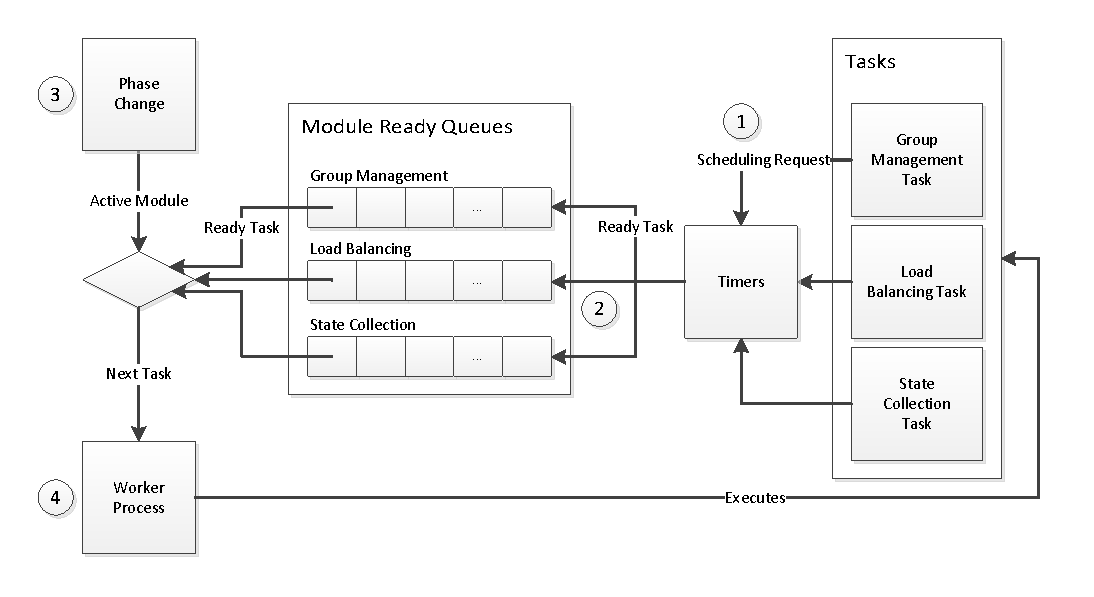
\includegraphics[width=1.0\textwidth]{RealTimeScheduler.pdf}
\captionsetup{singlelinecheck=off}
\caption[Real Time Scheduler]{The real time scheduler uses a round robin approach to allot execution time to modules. 
\begin{enumerate}
    \item Modules request that a task be executed by specifying a time in the
          future to execute a task. A timer is set to count down to the
          specified moment. Modules may also place tasks immediately into the
          ready queue if the task may be executed immediately.
    \item When the timer expires the task is placed into the ready queue for
          the module that requested the task be executed.
    \item Modules are assigned periods of execution (called phases) which are
          a predetermined length. After the specificed amount of time has
          passed, the module's phase ends and the next module in the schedule's
          tasks begin to execute.
    \item The worker selects the next ready task for the active module from the
          ready queue and executes it. These tasks may also schedule other tasks
          to be run in the future.
\end{enumerate}
}
\label{fig:REALTIMESCHEDULER}
\end{figure}

Modules inform the scheduler of tasks it wishes to perform by either submitting
them to be performed at some point in the future, or informing the scheduler of
a tasks that is ready to be executed immediately.

Tasks that have become ready, either by being inserted as ready, or the time
period that specified when it should be executed after has passed. The prepared
task is inserted into a ready queue for the module that the task has been
scheduled for.

When that modules phase is active, the task is pulled from the ready queue and
executed. When the phase is complete, the scheduler will stop pulling tasks
from the previous modules queue and begin pulling from the next modules queue.

This allows enforcement upper bound message delay. The modules have a specific
amount of processing time allotted. Modules with messages that invoke responses
(or a series of queries and responses) typically are required to be received
within the same phase, using round numbers which enforce that the message was
sent within the same phase.

Modules are designed and allotted time to allow for parameters such as maximum
query-response time (based on the latency between communicating processes). 
This implies that a module which engages in these activities has an
upper-bound in latency before messages are considered lost.
\section{Group Management Algorithm}

The DGI uses the leader election algorithm, ``Invitation Election
Algorithm'' written by Garcia-Molina in \cite{INVITATIONELECTION}.
Originally published in 1982, his algorithm provides a robust election
procedure which allows for transient
partitions. Transient partitions are formed when a faulty link between two or
more clusters of DGIs causes the groups to temporarily divide. These transient
partitions merge when the link is more reliable. The election algorithm
allows for failures that disconnect two distinct sub-networks. These sub
networks are fully connected, but connectivity between the two sub-networks is
limited by an unreliable link.

Since Garcia-Molina's original publication, there has been a large body of
work creating various election algorithms. Each algorithm is
designed to be well suited to the circumstances it will deployed in: there are
specialized algorithms for wireless sensor
networks\cite{LE-WSN-1}\cite{LE-WSN-2}, detecting failures in
certain
circumstances\cite{LE-SPECIALCIRCUMSTANCES-1}\cite{LE-SPECIALCIRCUMSTANCES-2}, and of course, transient partitions. Work on leader
elections has been incorporated into a variety of distributed frameworks:
Isis\cite{ISISTOOLKIT},
Horus\cite{HORUSTOOLKIT}, Totem\cite{TOTEMTOOLKIT},
Transis\cite{TRANSISTOOLKIT}, and Spread\cite{SPREADTOOLKIT} all have methods for creating groups. Despite
this wide body of work, the fundamentals of leader election are consistent
across all work: nodes arrive at a consensus of a single peer who coordinates
the group, and nodes the fail are detected and removed from the group.

The elected leader is responsible for making work assignments and identifying 
and merging with other coordinators when they are found, as well as maintaining 
a up-to-date list of peers for the members of his group.  Likewise, members of 
the group can detect the failure of the group leader by periodically checking 
if the group leader is still alive by sending a message. If the leader fails to 
respond, the querying node will enter a recovery state and operate alone until 
they can identify another coordinator to join with. Therefore, a leader and each
of the members maintains a set of processes which are currently reachable, which
is a subset of all known processes in the system.

This Leader election can also be classified as a failure detector 
\cite{LEADERELECTIONEVAL}. Failure detectors are algorithms which detect the failure of processes in a 
system. A failure detector algorithm maintains a list of processes that it suspects have
crashed. This informal description gives the failure detector strong ties to the
Leader Election process. The Group Management module maintains a list of 
suspected processes which can be determined from the set of all processes and the current
membership. 


The leader and members have separate roles to play in the failure detection
process. Leaders use a periodic search to locate other leaders in order to merge groups.
 This serves as a ping / response query for
detecting failures in the system. It is also capable of detecting a change in state either
by network issue or crash failure that causes the process being queried to no
longer consider itself part of the leader's group. The member will only suspect the leader, and not the other processes.
Of course, simple modifications could allow the member to suspect other members
by use of a heart beat or query-reply system, but it is not implemented in DGI code.

In this work it is assumed that a leader does not span two partitioned networks:
if a group is able to form, all members have some chance of communicating with
each other.


In this work it is assumed that a leader does not span two partitioned networks:
if a group is able to form all members have some chance of communicating with
each other.

\section{Network Simulation}

Network unreliability is simulated by dropping datagrams from specific sources 
on the receiver side. Each receiver was given an XML file describing the 
prescribed reliability of messages arriving from a specific source. The 
network settings were loaded at run time and could be polled if necessary for 
changes in the link reliability.

On receipt of a message, the broker's communication layer examine the source 
and select randomly based on the reliability prescribed in the XML file whether 
or not to drop a message. A dropped message was not delivered to any of the 
sub-modules and was not acknowledged by the receiver. Using this method we were 
able to emulate a lossy network link but not one with message delays.


\section{Markov Models}

Markov models are a common way of recording probabilistic processes that can
be in various states which change over time. A Markov model is a directed
graph composed of states, and transitions between these states. Each
transition has some probability attached to them.

Since the system, taken as a whole, can be reasonably modeled as a collection of
states each describing the state or configuration of the system, and that the
transitions between those state (failure events or election events) are probabilistic,
rather than deterministic, it is a natural extension to model the distributed
system as a Markov Chain.

\subsection{Continuous Time Markov Chains}

The models begins in some initial state, and then transitions into other states
based on the probabilities assigned on each edge of the graph. Each state is
memoryless, meaning that the history of the system, or the previous states have
no effect on the next transition that occurs. Letting $Fx(s)$ equal the complete
history of a Markov chain $X$ up to time $s$, and letting $j \in S$, where $S$
is the complete set of states in the model.

\begin{equation}
P\{ X(t)=j | F_X(s) \} = P\{ X(t)=j | X(s) \}
\end{equation}

Additionally, the models we present are time homogeneous, meaning that the
time that transition probabilities are not affected by the amount of time that
has passed in the simulation. CITE STOICH BIO

\begin{equation}
P\{ X(t)=j | X(s) \} = P\{ X(t)=j | X(0) \}
\end{equation}

Models can be either discrete time or continuous time. In a discrete time model
time is divided into distinct slices. After each "slice" the system transitions
based on the random chance from each of possible transitions. The discrete model
also allows for a transition which returns to the same state.

To contrast, a continuous time model assumes that the time between transitions
are exponentially distributed. Each transition has some expected value or mean
value which describes the amount of time before a transition occurs. Continuous
time models do not have transitions which return to the same state since the
expected value of the transition time describes when how long the system 
remains in the same state The probability density
function (PDF) of the exponential distribution can be written as: CITE

\begin{equation}
f(x;\lambda) = \begin{cases}
\lambda e^{-\lambda x} & x \ge 0 \\
0, & x < 0
\end{cases}
\end{equation}

As a result, the expected or mean value of an exponential distribution, is a function of
the parameter $\lambda$: CITE

\begin{equation}
\mathrm{E}[X] = \frac{1}{\lambda}. \!
\end{equation}

When there are multiple possible transitions from a state, each with their own
expected transition time, the expected amount of time in the state is:

\begin{equation}
\sum \lambda(x,y) = \sum \lambda p_{x,y} = \lambda(x)
\end{equation}

Where lambda(x,y) is the expected amount of time before state $x$ transitions to
state $y$. Interestingly, the expected time in a state ($\lambda(x)$) is related
to a the expected time for an individual transition ($\lambda(x,y)$) by a probability
$p_{x,y}$.

Each transition lends to an expected amount of time expected in the state. Then,
to do a random walk of a continuous time Markov chain, an intensity matrix must
also be generated in order to describe which transition is taken after the
exponentially distributed amount of time in the state has passed. Consider then
two streams of random variables, one of which is exponentially distributed and
used to determine the amount of time in a state. The second stream is normally
distributed and used to determine which state to transition to through the
intensity matrix.

\subsection{Assumptions}
In order to model the system, we assumed that the time between events was
exponentially distributed. Furthermore, we assumed that the system would be
fairly well synchronized, with most elections occurring at the same time. This
assumption was valid for 2-Node cases of our non-real-time code, but was
a major issue as the number of nodes began to increase. However, with of
the use of the round-robin scheduler with synchronization to enforce our
real-time requirements, assuming the synchronization of processes is not a
major leap.

All participating peers are assumed to be on the same schedule: all
peers begin execution of a model simultaneously. This is accomplished using \cite{DCS}.
This work assumes that the clocks are synchronized: even if the network has faulted,
process clocks have not drifted noticeably from their last synchronization. Additionally,
a production system would likely use GPS time synchronization in order to take
certain power system readings \cite{PHASORREADINGS}.

\subsection{Constructing The Markov Chain}

Consider a set of processes, which are linked by some packet based network
protocol. In our experiments we provide two protocols, each with different
delivery characteristics. Under ideal conditions a packet sent by one process
will always be delivered to its destination. Without a delivery protocol, as
soon as packets are lost by the communication network, the message that it
contained is lost forever. Therefore to compensate for the network losing
packets, a large variety of delivery protocols have been adapted. Each protocol
has a different set of goals and objectives, depending on the application.

Keeping in mind that a single lost packet does not necessitate the message it
contained is forever lost, different protocols allow for different levels of
reliability despite packet loss.

The leader election algorithm is centered around two critical events: checking,
and elections. The check system is used to detect both failures and the
availability of nodes for election. Processes in the system occasionally exchange
messages to determine if the other processes have crashed, and to discover new
leaders.

The DGI can perform work assuming that it is in a group, and not in an election
state (since the group management module instructs other modules to stop during
an election). The collected data in the previous sections is based on that
assumption, and the Markov chains that models those scenarios needed to as
well.

Processes in the DGI are either members or leaders. Leaders are processes
which have won elections among its members.

As stated previously, it was assumed that the events in the distributed system
were distributed exponentially. Events are modeled in the chain
using $\lambda(x)$ which is the parameter of the exponential distribution. It
is important to note that:

\begin{equation}
\mathrm{E}[X] = \frac{1}{\lambda}. \!
\end{equation}

and

\begin{equation}
\lambda(x) = \sum \lambda(x,y) = \sum \lambda(x) p(x,y)
\end{equation}

Where $\lambda(x)$ is the exponential parameter for the total time spend in
a state $x$, $\lambda(x,y)$ is the exponential parameter for a transition from
state $x$ to state $y$, and $p(x,y)$ is the normally distributed probability that
a state transitions from state $x$ to state $y$.

\subsubsection{Failure Detection}
When a leader sends its check messages, the nodes that receive it either
respond in the positive, indicating that they are also leaders, or in the
negative indicating that they have already joined a group. This message is sent
to all known nodes in the system. If a process replies that it is also a
leader, the original sender will enter and election mode and attempt to combine
groups with the first process. Nodes that fail to respond are removed from the
leaders group, if they were members.

The member on the other hand will only direct its check message to the leader
of its current group. As with the leader's check message, the response can
either be positive or negative. A ``yes'' response indicates that the leader is
still available and considers the member a part of its group. A ``no'' response
indicates that either the leader has failed and recovered, or it has suspected
the member process of being unreachable (either due to crash or network issue)
and has removed them from the group. In this event the member will enter a
recovery state and reset itself to an initial configuration where it is in a
group by itself.

On any membership change, either due to recovery, or a suspected failure, the
list of members for a group is pushed to every member of that group by the
leader. Members cannot suspect other processes of being crashed, only the
leader can identify failed group members.

\begin{figure*}
\centering
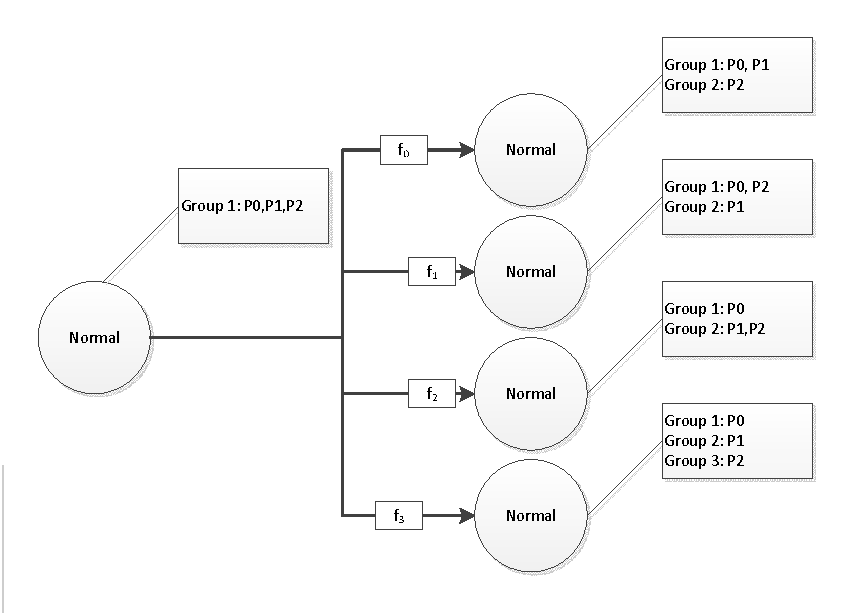
\includegraphics[width=.9\linewidth]{markov-ayc.pdf}
\caption{A diagram showing a partial Markov chain for failure detection}
\label{fig:MARKOVAYC}
\end{figure*}

A model of a failure detection stage of the leader election algorithm is presented in
Figure \ref{fig:MARKOVAYC}. A set of nodes begin in a normal state as part of a group.
The leader sends a query to every member, and every member sends a query to the leader.
If a response is not received in either direction, the process is considered to be
unreachable and is either ejected from the group by the leader (if the query originated from the leader)
or the member leaves the group and becomes a coordinator themselves.

The system will stay in the original state as long as all nodes complete their queries and responses.
Let $T_{R}$ be the amount of time allowed for a response, $T_{C}$ be the time between
discovery attempts, and $p_{F}$ is the probability that at least one peer fails to complete the exchange.
Based on this, the expected amount of time in the grouped state ($T_{G}$) is:

\begin{equation}
\begin{cases}
T_{G} = ( T_{R}+T_{C}  ) / p_{F} & p_{F} > 0 \\
\infty & p_{F} = 0
\end{cases}
\end{equation}

Let $\delta$ equal exponential parameter of the exponential distribution for the base state. Then
we can relate the probabilities of each possible transition to the parameter for the base state. Let
$p_{i}$ be the probability of transitioning to configuration $i$ after leaving the base state and let
$f_{i}$ be the exponential parameter for the transition to an individual configuration:

\begin{equation}
\delta = \sum f_{i} = \sum \delta p_{i} = \frac{1}{T_{G}}
\end{equation}


\subsubsection{Leader Election}
During elections, a highest priority leader (identified by its process id) will
send invites to the other leaders it has identified. If those leaders accept
the highest priority leader's invites, they will reply with an accept message
and forward the invite to their members, if their are any. If the highest
priority process fails to become the leader the next highest will send invites
after a specified interval has passed.

Therefore, the membership of the system can be affected in two ways: election
events which change the size of groups and failure suspicion (via checks) which
decreases the size of groups. Note that elections can decrease the size of
groups as well as increase them: If a round of forwarding invites fails by the
new leader to his original group, the group size could decrease.

When a process is initialized it begins in the ``solo'' state: it is in a group
with itself as the only member. As nodes are discovered by checks, the
processes combine into groups. Groups are not limited by increasing one a time;
they can increase by combined size of the groups of the leader processes.

We define a metric to assess the performance of the system under duress: we
first consider that the distributed can only perform meaningful work when the
processes can work together to perform physical migration. This means that
there are two networks that affect the system's ability to do work: the
physical flow network and the cyber communication network.


\begin{figure}[!h]
\centering
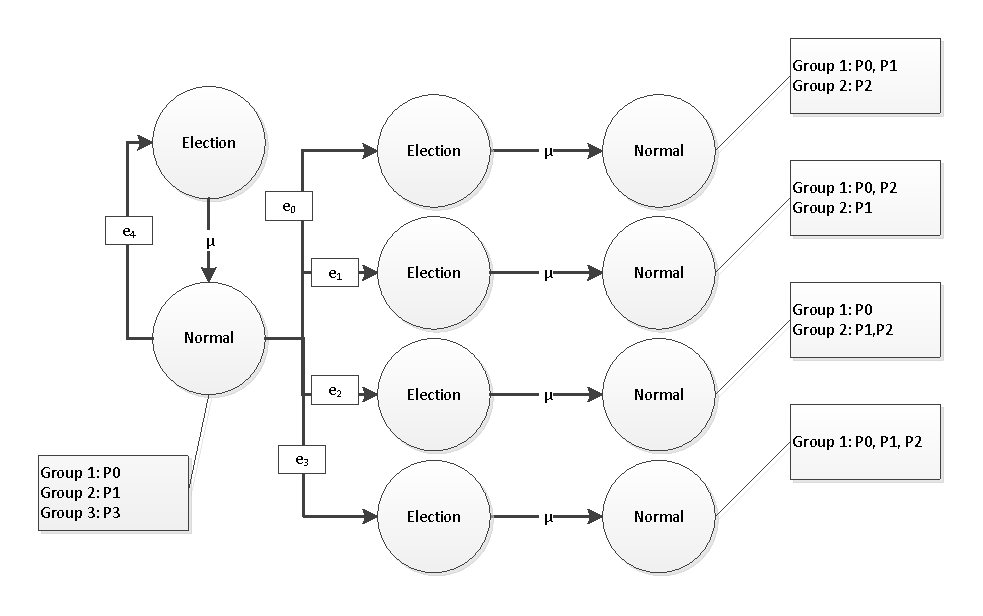
\includegraphics[width=1.0\linewidth]{markov-election.pdf}
\caption{A diagram showing a partial Markov chain for an election}
\label{fig:MARKOVELECTION}
\end{figure}

A continuous time Markov model of a single election is presented in Figure \ref{fig:MARKOVELECTION}.
A set of leaders begin in a normal state. After some time $T_{D}$ an ``are you coordinator''
message discovers some other peer. $T_{D}$ is a function of the number of discovery
checks which discover no leaders (which in turn is a function of the link reliability). Let
$T_{R}$ be the amount of time allowed for a response, $T_{C}$ be the time between
discovery attempts, and $p_{D}$ is the probability that the exchange discovers a leader.

\begin{equation}
\begin{cases}
T_{D} = ( T_{R}+T_{C} ) / p_{D} & p_{D} > 0 \\
\infty & p_{D} = 0
\end{cases}
\end{equation}

Then, the parameters $e_x$ in Figure \ref{fig:MARKOVELECTION} are a function of $T_{D}$ and $p_{x}$,
the probability an election results in configuration $x$.

\begin{equation}
e_x = \frac{p_{x}}{T_{D}}
\end{equation}

Once a leader has been discovered, the system transitions into an election state, based on the
potential outcome, where the peers hold an election to determine a new configuration. As shown
in Figure \ref{fig:MARKOVELECTION}, an election can either succeed or fail, resulting in a new system
configuration, or each involved process to return to the single member group state.

The amount of time that an election takes is fixed before the algorithm is executed.
Let $T_{E}$ be the mean time it takes to complete any election. Therefore:

\begin{equation}
\mu = \frac{1}{T_{E}}
\end{equation}

\subsubsection{Combined Model}

A combined model combines election and failure detection Markov chain components. Except for the
states where all reachable nodes are in the same group and the states where there are no reachable
leaders each state has a combination of election transitions and failure transitions.                           
The combined model is predictive of the overall characteristics of the system. The
time spent in a particular configuration is a function of the $\lambda$'s of all the
events that can cause the system to transition away from a configuration.

To construct the Markov chain, simulations of individual events are performed. The circumstances
for the events are assumed to be homogeneous: processes only differ by their process id.
Using this assumption, the simulation of events can be broken down into a series of scenarios
that are representative of the events in the system. Since each scenario is independent of other
scenarios, each scenario can be run independently.  Additionally, since the circumstances
are assumed to be homogeneous, scenarios that are similar, such as ones where two processes
swap roles can be simulated only once, and the results can be transformed from one scenario
to another with a simple mapping. This mapping scheme and parallizability helps keep the
state space explosion of the potential states under control.

